\section{E-Mail}
\begin{frame}{E-Mails: Was soll geschützt werden?}
  E-Mails können
  \begin{itemize}
    \item abgehört
    \item gefälscht
  \end{itemize}
  werden. Deshalb stellen wir vor, wie man
  \begin{itemize}
    \item die Vertraulichkeit (das ,,Briefgeheimnis``) umsetzt
    \\ $\Rightarrow$ Verschlüsselung
    \item die Echtheit des Gegenübers sicherstellt
    \\ $\Rightarrow$ Digitale Signatur
  \end{itemize}
  Außerdem:
  \begin{itemize}
    \item Wie man sicherstellt, dass sein E-Mail Passwort\\ nicht einfach mitgelesen werden kann
  \end{itemize}
\end{frame}

\begin{frame}{E-Mail}{Funktionsweise}
  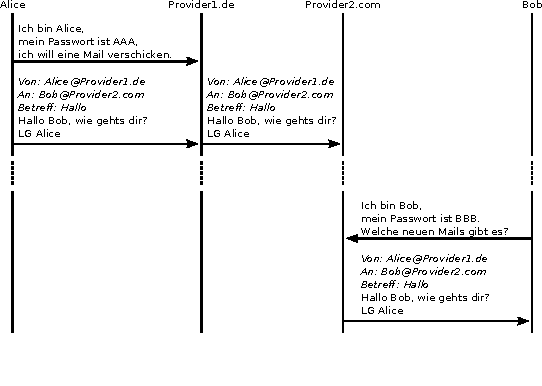
\includegraphics[width=.9\textwidth]{images/maildaten.pdf}
  \scriptsize
  ~\\
  ~\\
\end{frame}

\begin{frame}{E-Mail}{Transportverschlüsselung}
  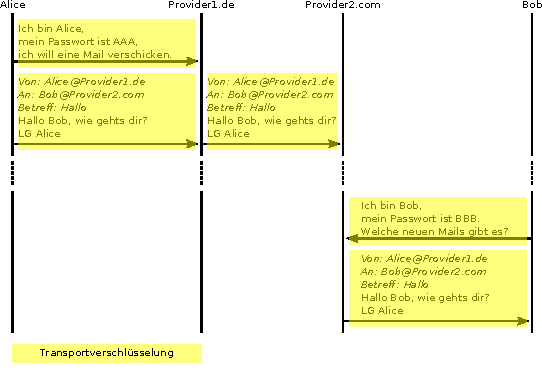
\includegraphics[width=.9\textwidth]{images/maildaten_trans.pdf}
  \begin{itemize}
    \scriptsize
    \item muss von den Mailanbietern unterstützt werden
    \item Konfiguration des Mailprogramms überprüfen!
  \end{itemize}
\end{frame}

\begin{frame}{E-Mail}{Ende-zu-Ende-Verschlüsselung}
  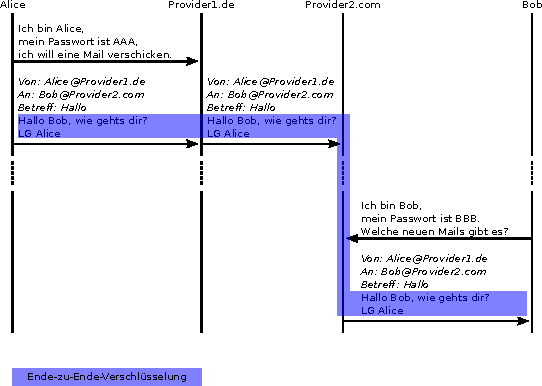
\includegraphics[width=.9\textwidth]{images/maildaten_e2e.pdf}
  \begin{itemize}
    \scriptsize
    \item unabhängig vom Mailanbieter möglich
    \item verhindert Mitlesen von Mail-\textbf{Nutzdaten}
  \end{itemize}
\end{frame}

\begin{frame}{E-Mail}{Kombination}
  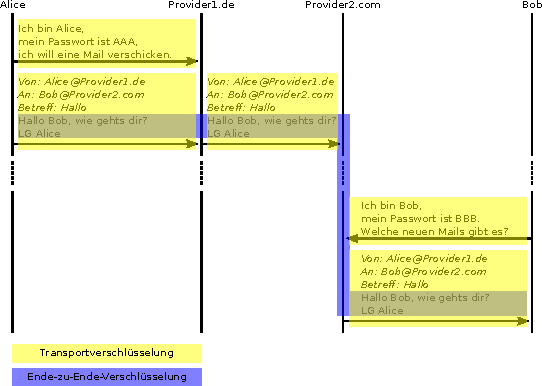
\includegraphics[width=.9\textwidth]{images/maildaten_beides.pdf}
  \scriptsize
  ~\\
  ~\\
\end{frame}
%\begin{frame}{Analogie zur Vertraulichkeit von E-Mails}
%  \begin{itemize}
%    %TODO: überarbeiten
%    \item E-Mails sind ,,Postkarten``
%    \item Transportiert in ,,gläsernen Fahrzeugen``
%    \begin{itemize}
%      \item ,,Autobahnbetreiber`` kann alles mithören
%      \item ,,Post`` kann alles mithören
%    \end{itemize}
%    \item Bei \emph{Transportverschlüsselung} ersetzt die ,,Post``\\ ,,gläserne Fahrzeuge`` durch ,,blickdichte Fahrzeuge``
%    \begin{itemize}
%      \item ,,Autobahnbetreiber`` kann mithören,\\ wann welche ,,Post`` mit welcher ,,Post`` redet\\ aber nicht Passwort, Empfänger, Betreff, etc.
%      \item ,,Post`` kann alles mithören
%    \end{itemize}
%    \item Bei \emph{Ende-zu-Ende-Verschlüsselung} steckt der Absender die ,,Postkarte`` in einen ,,Briefumschlag``
%    \begin{itemize}
%      \item ,,Autobahnbetreiber`` und ,,Post`` können mithören,\\ wann wer mit wem wie viel kommuniziert\\ aber nicht den Inhalt!
%    \end{itemize}
%    \item Unbedingt beides kombinieren!
%  \end{itemize}
%\end{frame}

\begin{frame}{Überprüfung der Echtheit}
Was, wenn A eine Nachricht an B schicken will,\\ aber den öffentlichen Schlüssel von B nicht kennt?\\
\begin{enumerate}
  \item Im ``Telefonbuch'' nach dem Schlüssel suchen
  \item Echtheit mit Hilfe eines \emph{vertrauenswürdigen Dritten} C überprüfen
\end{enumerate}
\begin{center}
  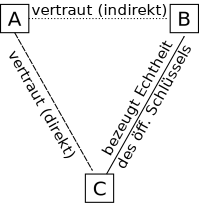
\includegraphics[width=0.5\textheight]{images/vertrauen.pdf}
  %TODO: überarbeiten
\end{center}
\end{frame}

\begin{frame}{Wie stellt man Vertrauen her?}
  \begin{itemize}
    \item S/MIME -- Hierarchischer Vertrauensansatz
    \begin{itemize}
      \item hier nicht behandelt
    \end{itemize}
    \item GnuPG -- Dezentraler Vertrauensansatz
    \begin{itemize}
      \item jeder kann festlegen, wem er vertraut
      \begin{itemize}
        \item er kann die Echtheit eines Schlüssels\\ z.B. bei einem persönlichen Treffen überprüfen
      \end{itemize}
      \item jeder \emph{kann} sein Vertrauensnetz veröffentlichen (Web-of-Trust)
      \begin{itemize}
        \item Vorteil: Man kann ``Freunden von Freunden'' vertrauen
        \item Nachteil: Beziehungen zwischen Menschen öffentlich\\ Aber: Facebook sagt da viel mehr aus
      \end{itemize}
      %\item wird hier behandelt
    \end{itemize}
  \end{itemize}
\end{frame}

\begin{frame}{Welche Software benötigt man?}
  \begin{block}{OpenPGP Backend}
    Macht die eigentliche Ver-/Entschlüsselung \& Signatur

    \vspace{1ex}
    \begin{tabular}{ccc}
      Linux:            & Windows: & Android:     \\
      \textit{on-board} & GPG4Win  & OpenKeychain \\
    \end{tabular}
  \end{block}
  \begin{block}{Plug-In fürs Mailprogram}
    Grafische Oberfläche, leichtere Schlüsselverwaltung, etc.

    \vspace{1ex}
    \begin{tabular}{ccc}
      Thunderbird: & Outlook: & K9-Mail: \\
      Enigmail     & GPG4Win  & --       \\
    \end{tabular}
  \end{block}
\end{frame}

\endinput
